% vim: fo=aw2tq tw=100
\documentclass[a4paper,10pt]{article}
\setlength{\parskip}{0.5\baselineskip}

% Necessary packages
\usepackage{pslatex}
\usepackage{listings}
\usepackage{shortvrb}
\usepackage[pdftex]{color,graphicx}
\usepackage[pdftex]{hyperref}

% Use "foo" for short verbatim
\MakeShortVerb{\"}

% Coloured links, not frames
\hypersetup{colorlinks=true}

% Define a listings language for h180
\lstdefinelanguage{h180}{
    keywordsprefix=.,
    keywords={add,adc,and,cp,cpl,dec,inc,mlt,neg,or,sub,sbc,tst,xor,rl,rla,rlc,rlca,rr,rra,rrc,
rrca,rld,rrd,sla,sra,srl,set,res,bit,ld,cpd,cpdr,cpi,cpir,ldd,lddr,ldi,ldir,push,pop,ex,exx,call,
djnz,jp,jr,ret,reti,retn,rst,in,in0,ind,indr,ini,inir,out,out0,otdm,otdmr,otdr,outi,otir,tstio,otim,
otimr,outd,daa,ccf,scf,di,ei,halt,im,nop,slp},
    sensitive=false,
    comment=[l]{\#},
}
% Define the h180 environment
\lstnewenvironment{h180}{\lstset{language=h180}}{}
% Define the global listing style
\lstset{lineskip=-1pt, basicstyle=\small\ttfamily, frame=lines, framerule=0.2pt}


% Document info
\title{Microcomputer Communications Project (MCP)}
\author{Examination number: Y2265520}

\begin{document}

% Title page
\maketitle
%\vfill
\begin{center}
1234 words
\end{center}
\pagebreak
% Table of Contents
\tableofcontents

\pagebreak
\section{Introduction}

The aim of the project is the development and implementation of an embedded system capable of 
synthesising one or more musical instruments, and playing these instruments in a real-time manner 
based on a serial network data stream.

The base hardware supplied for this task is a Single-Board Computer (SBC) based on the Hitachi 64180 
CPU - a Z180 clone, which in turn is an extended Z80, with a few extra instructions and most of the 
useful peripherals built in (serial I/O controller, DMA controller, programmable reload timers).  
This CPU is clocked faster than the Z80, at 6.144MHz, and has a physical address space of 512kB 
courtesy of a programmable Memory Management Unit (MMU), but shares the Z80's 64kB logical address 
space since the instruction set only allows 16-bit memory addresses.  Some instructions have also 
been implemented more efficiently, requiring fewer clock cycles to complete.

In addition to the 64180 chip, many other useful peripherals are part of the SBC, including an 
I$^{2}$C controller, Real-Time Clock (RTC), 24-bit parallel digital I/O, 4-bit hexadecimal keypad 
and 16*2 character LCD text display.  The board is fitted with 96kB of RAM, and a ROM containing a 
very basic operating system that, among other things, supports loading software over a serial 
connection and starting execution at a specified memory location.

% TODO: More info on the output
Output is to be via a supplied $8\Omega$ impedance speaker.  Any other hardware required for the 
output is to be designed and built jointly with a partner, since repeated changing of hardware on a 
shared system for testing individual solutions is impractical, and the design of the hardware will 
heavily influence the way in which the software is written.

\pagebreak
\section{Functional Overview}

\begin{figure}[!htbp]
\centering
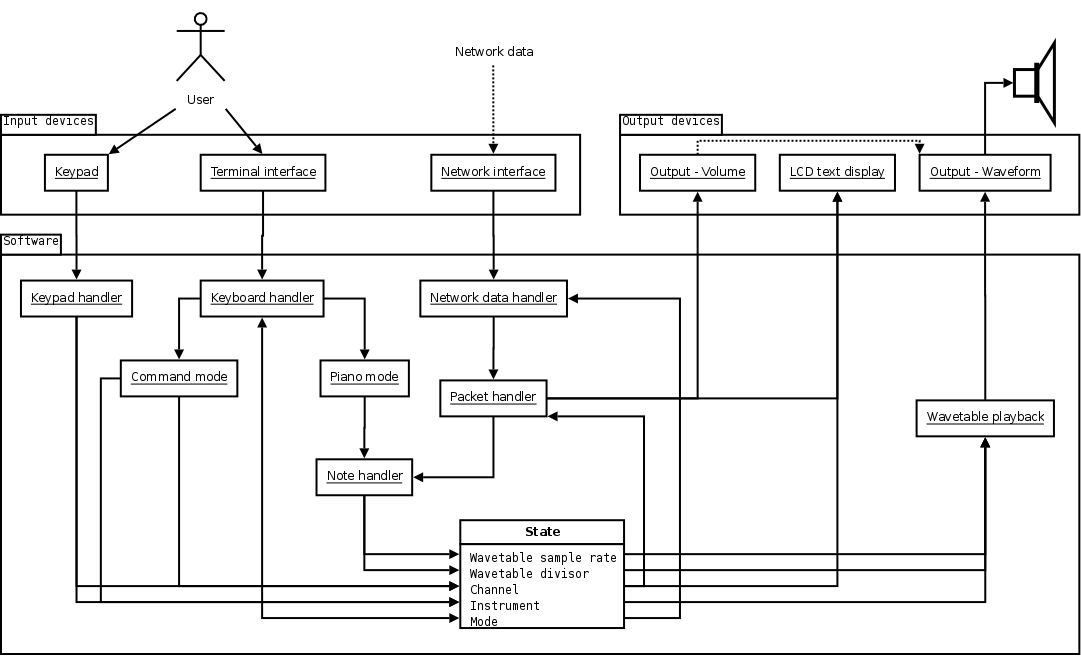
\includegraphics[totalheight=0.55\textheight,angle=90]{images/overview.png}
\caption{System overview}\label{fig:systemoverview}
\end{figure}

The diagram in Figure \ref{fig:systemoverview} shows the conceptual architecture of my system.  The 
basic idea is that various inputs are processed and in some way modify the state of the system, and 
this state in turn affects the operation of the continuously-running wave table playback.

The most important element of the system is the real-time conversion of network data into

\pagebreak
\section{Design and Implementation}

\pagebreak
\section{Testing and Evaluation}

\pagebreak
\section{Technical Specification}

\pagebreak
\section{Further Work}


\appendix

\pagebreak
\begin{thebibliography}{99}
% \bibitem{ref}Author:
% \emph{Title},
% \url{http://} (year)
\end{thebibliography}

\end{document}
